\documentclass[10pt,t]{beamer}


\setbeamersize{text margin left=10pt,text margin right=10pt}
\usetheme{lehigh}

\usefonttheme{professionalfonts}
\usefonttheme{serif}

% add packages to use
\usepackage{tabularx}
\usepackage{tikz}
\usetikzlibrary{trees,matrix,shapes,arrows}
\usetikzlibrary{calc}
\usepackage{fancyvrb}
\usepackage{listings}

\pgfdeclarelayer{background}
\pgfdeclarelayer{foreground}
\pgfsetlayers{background,main,foreground}
\usepackage[latin1]{inputenc}
\usepackage[english]{babel}
\usepackage{hyperref}
\usepackage[normalem]{ulem}

                                                         
%\usepackage{times}
%\usepackage[T1]{fontenc}
\usepackage{graphicx}
%\usepackage{pgf,pgfarrows,pgfnodes,pgfautomata,pgfheaps,pgfshade}
\usepackage{amsmath,amssymb,amsfonts,subfigure,pifont}
\usepackage{multirow}
\usepackage{booktabs}
\usepackage{colortbl}
\usepackage{keystroke}
\usepackage{etex}


% The following color are for listing environment 
\definecolor{dkgreen}{rgb}{0,0.6,0}
%\definecolor{gray}{rgb}{0.5,0.5,0.5}
\definecolor{mauve}{rgb}{0.58,0,0.82}


\lstset{%
language=bash,                % the language of the code
basicstyle=\tiny\ttfamily,           % the size of the fonts that are used for the code
showspaces=false,               % show spaces adding particular underscores
showstringspaces=false,         % underline spaces within strings
showtabs=false,                 % show tabs within strings adding particular underscores
%frame=single,                   % adds a frame around the code
%rulecolor=\color{black},        % if not set, the frame-color may be changed on line-breaks within not-black text (e.g. comments (green here))
tabsize=2,                      % sets default tabsize to 2 spaces
%captionpos=b,                   % sets the caption-position to bottom
breaklines=true,                % sets automatic line breaking
breakatwhitespace=false,        % sets if automatic breaks should only happen at whitespace
%title=\lstname,                   % show the filename of files included with \lstinputlisting;
% also try caption instead of title
keywordstyle=\color{blue},          % keyword style
commentstyle=\color{dkgreen},       % comment style
stringstyle=\color{mauve},         % string literal style
escapeinside={!}{!},            % if you want to add LaTeX within your code
morekeywords={*,\dots,elif},              % if you want to add more keywords to the set
deletekeywords={\dots},              % if you want to delete keywords from the given language
%morecomment=[l]{//}
}
\lstset{%
language=csh,                % the language of the code
basicstyle=\tiny\ttfamily,           % the size of the fonts that are used for the code
showspaces=false,               % show spaces adding particular underscores
showstringspaces=false,         % underline spaces within strings
showtabs=false,                 % show tabs within strings adding particular underscores
%frame=single,                   % adds a frame around the code
%rulecolor=\color{black},        % if not set, the frame-color may be changed on line-breaks within not-black text (e.g. comments (green here))
tabsize=2,                      % sets default tabsize to 2 spaces
captionpos=b,                   % sets the caption-position to bottom
breaklines=true,                % sets automatic line breaking
breakatwhitespace=false,        % sets if automatic breaks should only happen at whitespace
%title=\lstname,                   % show the filename of files included with \lstinputlisting;
% also try caption instead of title
keywordstyle=\color{blue},          % keyword style
commentstyle=\color{dkgreen},       % comment style
stringstyle=\color{mauve},         % string literal style
escapeinside={\%*}{*)},            % if you want to add LaTeX within your code
morekeywords={*,\dots,elif},              % if you want to add more keywords to the set
deletekeywords={\dots},              % if you want to delete keywords from the given language
%morecomment=[l]{//}
}

\lstdefinestyle{LINUX}
{
    backgroundcolor=\color{white},
    basicstyle=\tiny\ttfamily,
    keywordstyle=\color{blue},
    morekeywords={apacheco,Tutorials,BASH,scripts,day1,examples},
    literate={>}{{\textcolor{blue}{>}}}1
         {/}{{\textcolor{blue}{/}}}1
         {./}{{\textcolor{black}{./ }}}1
         {~}{{\textcolor{blue}{\textasciitilde}}}1,
}



\DeclareSymbolFont{extraup}{U}{zavm}{m}{n}
%\DeclareMathSymbol{\vardiamond}{\mathalpha}{extraup}{87}
\newcommand{\cmark}{\ding{51}}
\newcommand{\xmark}{\ding{55}}
\newcommand{\smark}{\ding{77}}
\newcommand*\vardiamond{\textcolor{lubrown}{%
  \ensuremath{\blacklozenge}}}
\newcommand*\mybigstar{\textcolor{lubrown!90!yellow}{%
  \ensuremath{\bigstar}}}
\newcommand*\up{\textcolor{green!80!black}{%
  \ensuremath{\blacktriangle}}}
\newcommand*\down{\textcolor{red}{%
  \ensuremath{\blacktriangledown}}}
\newcommand*\const{\textcolor{darkgray}%
  {\textbf{--}}}
\newcommand*\enter{\tikz[baseline=-0.5ex] \draw[<-] (0,0) -| (0.5,0.1);}

\newcommand{\Verblubrown}[1]{\Verb[formatcom=\color{lubrown},fontseries=b,commandchars=\\\{\}]|#1|}
\newcommand{\Verblue}[1]{\Verb[formatcom=\color{lublue},fontseries=b,commandchars=\\\{\}]!#1!}
\newcommand{\Verbblue}[2][b]{\Verb[formatcom=\color{lublue},fontshape=#1,commandchars=\\\{\}]|#2|}
\newcommand{\Verblubrownp}[1]{\Verb[formatcom=\color{lubrown},fontseries=b,commandchars=\\\{\}]!#1!}


% LOGOS
% footer logo
\pgfdeclareimage[width=0.3\paperwidth]{university-logo}{lulogo}
\tllogo{\pgfuseimage{university-logo}}

%titlepage logo
\titlegraphic{\includegraphics[scale=0.5]{lu}}


\beamertemplateballitem
\usetikzlibrary{mindmap,trees}
\usetikzlibrary{decorations.text,calc,arrows.meta}

\definecolor{luorange}{RGB}{255,196,35}
\definecolor{luorange2}{RGB}{255,226,147}

%% Tikz Distro Watch Table
% Defining some symbols:
\newcommand*\head[1]{\textbf{#1}}
% The table environment:
\newenvironment{matrixtable}[4]{%
  \begin{tikzpicture}[matrix of nodes/.style={
    execute at begin cell=\node\bgroup\strut,
    execute at end cell=\egroup;}]
  \matrix (m) [matrix of nodes,top color=blue!20,
    bottom color=blue!80,draw=white,
    nodes={draw,top color=blue!10,bottom color=blue!35,
    draw,inner sep=2pt,minimum height=3.1ex},
    column sep=1ex,row sep=0.6ex,inner sep=2ex,
    rounded corners,column 1/.style={minimum width=#1},
    column 2/.style={minimum width=#2},
    column 3/.style={minimum width=#3},
    column 4/.style={minimum width=#4}]}%
{;\end{tikzpicture}}

\title{A Brief Introduction to Linux}
\subtitle{What is it? What can I use it for?}
\author{Alexander B. Pacheco}
\institute{\href{http://researchcomputing.lehigh.edu}{LTS Research Computing}}%\\[2pt] \href{http://www.lehigh.edu}{Lehigh University}}
\date{September 8, 2015}

% Delete this, if you do not want the table of contents to pop up at
% the beginning of each subsection:
\AtBeginSection[]
{
  \begingroup
  \setbeamertemplate{background canvas}[vertical shading][bottom=lubrown,top=lubrown]
  \setbeamertemplate{footline}[myfootline] 
  \setbeamertemplate{section page}[mysection]
  \frame[c]{
    \sectionpage
  }
  \endgroup
}

\titlegraphic{\includegraphics[scale=0.5]{lu}}
\begin{document}

\begin{frame}[c]
  \titlepage
\end{frame}

\footnotesize
\begin{frame}{Outline}
  \tableofcontents
\end{frame}

%\section*{Installing Linux on VirtualBox}
%\begin{frame}[fragile]
%  \frametitle{Installing Linux on VirtualBox}
%  \begin{enumerate}
%    \item Download and install Oracle VirtualBox (and the extension pack) from \href{https://www.virtualbox.org/wiki/Downloads}{here}
%    \item Download the CentOS virtual image from \href{https://drive.google.com/open?id=0ByziB2zqYhHVcHRKTWZqdFZUX0E&authuser=1}{here}. (you need to logged into Lehigh Google to access the image name CentOS.ova. Its about 2.6GB.)
%    \item Install the image by double clicking on it. If it doesn't work, open virtualbox software that you just installed, 
%    \begin{enumerate}
%      \item From the menu, click File$>$Import Appliance
%      \item Choose the ova file that you just downloaded and click the next button (this instruction may differ on Windows and Mac systems)
%      \item Click the import button
%    \end{enumerate}	
%    \item Whole process should take a few minutes.
%    \item Once the process is complete, you should see CentOS listed in the left sidebar.
%    \item Select CentOS and click the start button or double click CentOS
%    \item After a minute or two you should a login prompt
%    \item Type user and hit enter
%    \item You should now see a prompt such as \Verb[formatcom=\color{lubrown},fontseries=b,commandchars=\\\{\}]|[user@localhost ~]\$|
%    \item Create a password by typing passwd and hit enter. You will be prompted to enter a password twice, you will not see any characters on the screen as you type.
%    \item Create a password for admin user by first logging in as root: type su - at the prompt and hit enter. Follow the previous step
%  \end{enumerate}
%\end{frame}

%\section*{Logging into a remote Linux server}
%\begin{frame}[fragile]
%  \frametitle{Logging into a remote Linux server}
%  \begin{itemize}
%    \item Mac OSX
%    \begin{enumerate}
%      \item Open the Terminal App
%      \item At the command prompt enter \Verblubrown{ssh user@remotehost}
%      \item[] \Verblubrown{user} is your username on the remote Linux server
%      \item[] \Verblubrown{remotehost} is the hostname or ip address of the remote Linux server
%      \item[e.g] To log into polaris \Verblubrown{ssh alp514@polaris.cc.lehigh.edu} 
%    \end{enumerate}
%    \item Windows
%    \begin{enumerate}
%      \item Download and install a ssh client such as \href{http://www.putty.org/}{putty} or \href{http://mobaxterm.mobatek.net/}{MobaXterm}
%      \item Open the client
%      \item Putty: Enter the hostname or ip address of the remote Linux server (make sure the SSH radio button is selected) $>$ Click open
%      \item MobaXterm: Click New Session $>$ Select SSH tab $>$ Enter hostname and username in the field provided $>$ Click on OK
%      \item When you are prompted for your password, you may not not see any characters on the screen.
%    \end{enumerate}
%  \end{itemize}
%\end{frame}

\section{Introduction to Linux}
\frame[allowframebreaks]{
  \frametitle{Unix History}
  \begin{itemize}
    \item Unix was conceived and implemented in 1969 at AT\&T Bell labs by  Ken Thompson, Dennis Ritchie, Douglas McIlroy, and Joe Ossanna.
    \item First released in 1971 and was written in assembler.
    \item In 1973, Unix was re-written in the programming language C by Dennis Ritchie (with exceptions to the kernel and I/O).
    \item The availability of an operating system written in a high-level language allowed easier portability to different computer platforms.
    \item The GNU Project, started in 1983 by Richard Stallman, had the goal of creating a ``complete Unix-compatible software system'' composed entirely of free software.
    \item 386BSD released in 1992 and written by Berkeley alumni Lynne Jolitz and William Jolitz. FreeBSD, NetBSD, OpenBSD and NextStep (Mac OSX) descended from this
    \item Andrew S. Tanenbaum wrote and released MINIX, an inexpensive minimal Unix-like operating system, designed for education in computer science
    \item Frustated with licensing issues with MINIX, Linus Torvalds, a student at University of Helsinki began working on his own operating system which eventually became the "Linux Kernel"
    \item Linus released his kernel for anyone to download and help further development.
	\end{itemize}
        \begin{exampleblock}{Linus's message to comp.os.minix on Aug 26, 1991}
		{\scriptsize
Hello everybody out there using minix -\\
I'm doing a (free) operating system (just a hobby, won't be big and professional like gnu) for 386(486) AT clones.  This has been brewing since april, and is starting to get ready.  I'd like any feedback on things people like/dislike in minix, as my OS resembles it somewhat (same physical layout of the file-system (due to practical reasons) among other things).\\
I've currently ported bash(1.08) and gcc(1.40), and things seem to work. This implies that I'll get something practical within a few months, and I'd like to know what features most people would want.  Any suggestions are welcome, but I won't promise I'll implement them :-)\\
Linus (email address)\\
PS.  Yes - it's free of any minix code, and it has a multi-threaded fs. It is NOT protable (uses 386 task switching etc), and it probably never will support anything other than AT-harddisks, as that's all I have :-(.\\
}
            {\fontsize{5}{7}\selectfont{\url{https://groups.google.com/forum/?fromgroups=\#!msg/comp.os.minix/dlNtH7RRrGA/SwRavCzVE7gJ}}}
      \end{exampleblock}
	  \begin{itemize}
    \item Linux is only the kernel, an Operating System also requires applications that users can use.
    \item combined with free software available from the GNU project gave birth to a new Operating System known as "GNU/Linux"
    \item GNU/Linux or simply Linux is released under the GNU Public License: Free to use, modify and distribute provided you distribute under the GNU Public License.\let\thefootnote\relax\footnote{\tiny http://en.wikipedia.org/wiki/Linux}
  \end{itemize}
  }
\frame[c]{
  \begin{center}
    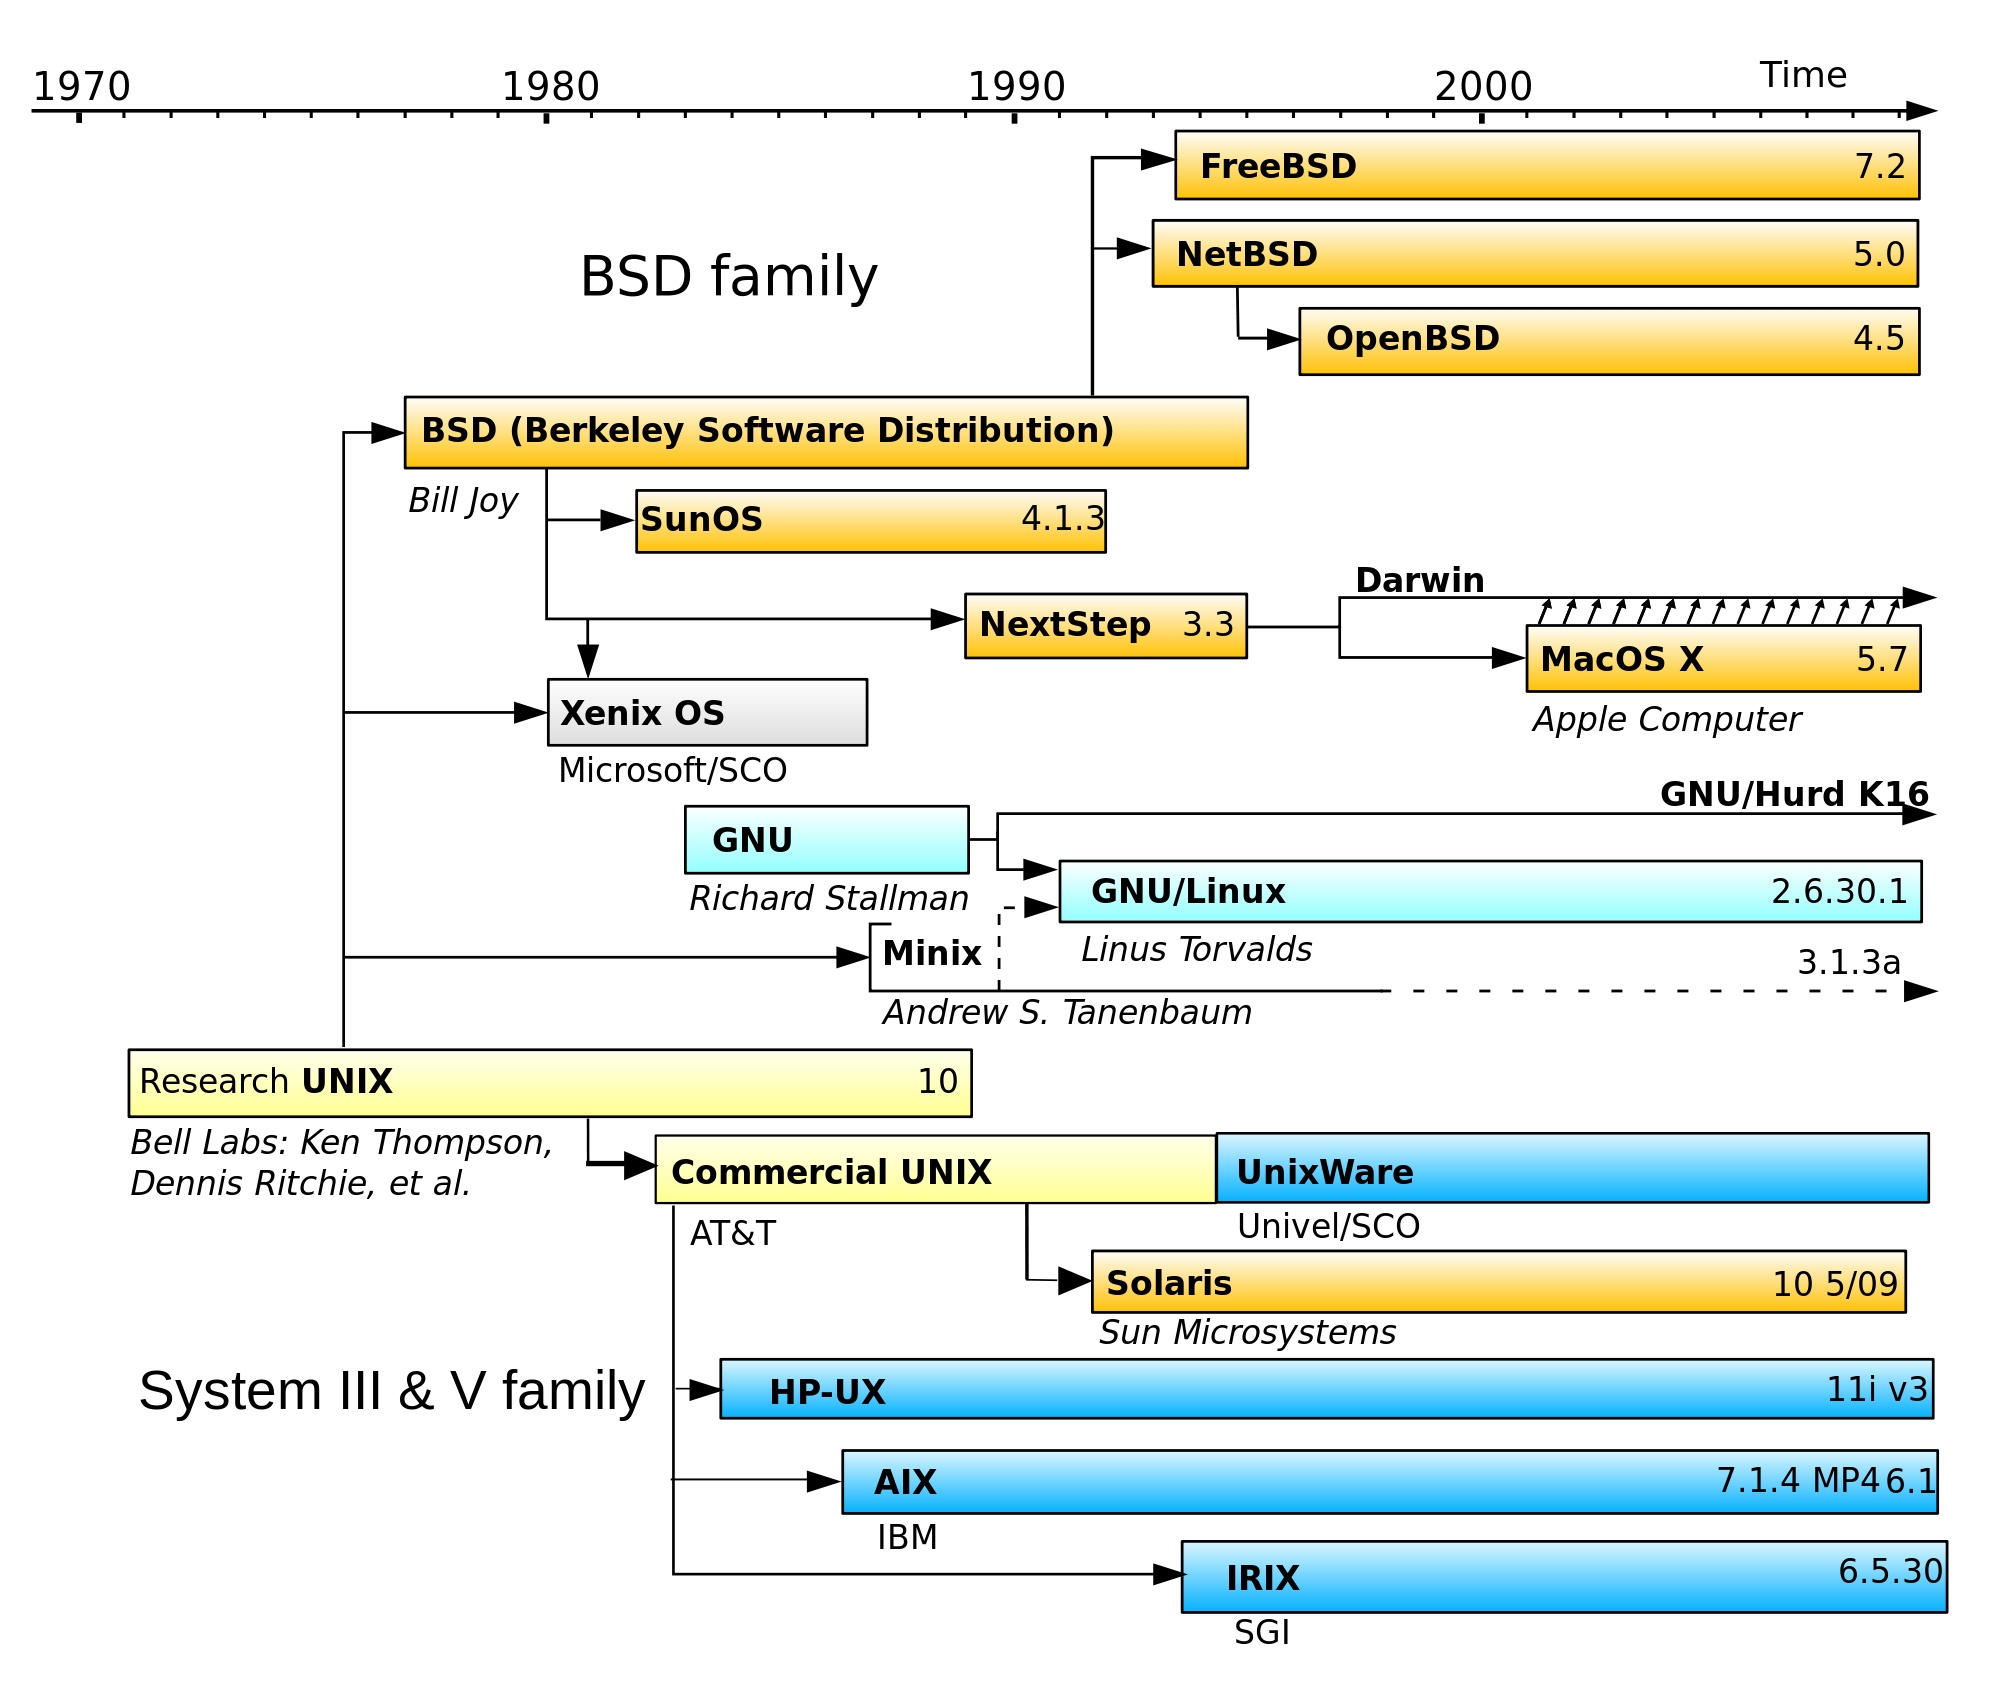
\includegraphics[width=0.8\textwidth]{./Unix_history}
  \end{center}
	}

\begin{frame}
  \frametitle{What is Linux?}
  \begin{itemize}
    \item Linux is an operating system that evolved from a kernel created by Linus Torvalds when he was a student at the University of Helsinki. 
    \item It's meant to be used as an alternative to other operating systems, Windows, Mac OS, MS-DOS, Solaris and others. 
    \item Linux is the most popular OS used in a Supercomputer\let\thefootnote\relax\footnote{\tiny \url{http://www.top500.org/statistics/list/}}\let\thefootnote\relax\footnote{\tiny June 2015 List}
      \begin{center}
  \begin{tikzpicture}
    \node (tbl) {
      \begin{tabularx}{0.42\textwidth}{ccc}
        \arrayrulecolor{black}
        \textcolor{white}{\textbf{OS Family} }& \textcolor{white}{\textbf{Count}} &\textcolor{white}{\textbf {Share \%}}\\
        Linux \rule{0pt}{3.5ex} & 489 & 97.8 \\
        Unix & 9 & 1.8 \\
        Windows & 1 & 0.2 \\
        Mixed & 1 & 0.2 \\
        [1.0ex]
    \end{tabularx}};
    \begin{pgfonlayer}{background}
      %\draw[rounded corners,top color=blue!30!black,bottom color=blue!10!white,
      \draw[rounded corners,top color=lupurple,bottom color=lupurple,
        draw=lubrown!30] ($(tbl.north west)+(0.14,0)$)
      rectangle ($(tbl.north east)-(0.13,0.9)$);
      %\draw[rounded corners,top color=green!5,bottom color=green!5,draw=green!5]
      \draw[rounded corners,top color=lulime,bottom color=lulime,draw=lulime]
      ($(tbl.north east)-(0.13,0.6)$)
      rectangle ($(tbl.south west)+(0.13,0.2)$);
    \end{pgfonlayer}
  \end{tikzpicture}
\end{center}



    \item If you are using a Supercomputer/High Performance Computer for your research, it will be based on a *nix OS.
    \item It is required/neccessary/mandatory to learn Linux Programming (commands, shell scripting) if your research involves use of High Performance Computing or Supercomputing resources.
  \end{itemize}
\end{frame}

\begin{frame}
  \frametitle{What is a Linux OS, Distro, Desktop Environment?}
  \begin{itemize}
    \item Many software vendors release their own packaged Linux OS (kernel, applications) known as distribution
    \item Linux distribution = Linux kernel + GNU system utilities and libraries + Installation scripts + Management utilities etc.
    \begin{enumerate}
      {%\scriptsize
        \item Debian, Ubuntu, Mint
        \item Red Hat, Fedora, CentOS
        \item Slackware, openSUSE, SLES, SLED
        \item Gentoo
      }
    \end{enumerate}
    \item Application packages on Linux can be installed from source or from customized packages
    \begin{enumerate}
      {%\scriptsize
        \item deb: Debian based distros e.g. Debian, Ubuntu, Mint
        \item rpm: Red Hat based distros, Slackware based distros.
      }
    \end{enumerate}
    \item Linux distributions offer a variety of desktop environment.
    \begin{enumerate}
      {%\scriptsize
        \item K Desktop Environment (KDE)
        \item GNOME 
        \item Xfce
        \item Lightweight X11 Desktop Environment (LXDE)
        \item Cinnamon
        \item MATE
        \item Dynamic Window Manager
      }
    \end{enumerate}
  \end{itemize}
\end{frame}

\begin{frame}
  \frametitle{Where is Linux used?}
  \begin{itemize}
    \item Linux distributions are tailored to different requirements such as
    \begin{enumerate}
      {%\scriptsize
        \item Server
        \item Desktop
        \item Workstation
        \item Routers
        \item Embedded devices
        \item Mobile devices (Android is a Linux-based OS)
      }
    \end{enumerate}
    \item Almost any software that you use on windows has a roughly equivalent software on Linux, most often multiple equivalent software
    \item[e.g.] Microsoft Office equivalents are OpenOffice.org, LibreOffice, KOffice
    \item For complete list, visit \url{http://wiki.linuxquestions.org/wiki/Linux_software_equivalent_to_Windows_software}
    \item Linux offers you freedom, to choose your desktop environment, software.
  \end{itemize}
\end{frame}

\begin{frame}[fragile]
  \frametitle{Popularity of Linux Distributions}
  \begin{columns}[T]
    \column{0.43\textwidth}
    \begin{itemize}
      \item \href{http://distrowatch.com/}{\color{blue}DistroWatch} provides news, popularity rankings, and other general information about:
      \begin{enumerate}
        {%\scriptsize
          \item various Linux distributions,
          \item free software/open source Unix-like operating systems such as OpenSolaris, MINIX and BSD.
        }
      \end{enumerate}
      \item DistroWatch is NOT an indication of market-share or quality nor is it an indication of how many users but  it is clearly an indication of what users are looking at.
    \end{itemize}
    \column{0.57\textwidth}
    \begin{center}
  {%\scriptsize
    \begin{matrixtable}{1.2cm}{2.4cm}{1.2cm}{0.6cm}{
        \head{Rank} & \head{Distribution} & \head{Hits} & \\
        1 & Mint        & 3105 & \const   \\
        2 & Debian      & 1764 & \up \\
        3 & Ubuntu      & 1603 & \const   \\
        4 & openSUSE    & 1198 & \up   \\
        5 & Fedora      & 1142 & \const   \\
        6 & Mageia      & 1016 & \down   \\
        7 & CentOS      & 970 & \down   \\
        8 & Manjaro     & 943 & \const \\
        9 & LXLE        & 788  & \up   \\
        10& Arch        & 759  & \const   \\
      }
    \end{matrixtable}
  }
\end{center}

  \end{columns}
\end{frame}

\section{Linux Components}
\begin{frame}[fragile]
  \frametitle{Linux Components}
  \begin{columns}[T]
    \column{0.55\textwidth}
%    \begin{itemize}
%    \item Linux is made up of two (three) parts:
      \begin{itemize}
      \only<1,2>{\item Kernel} 
      \only<1,3>{\item Shell}
      \only<1,4>{\item Applications/Programs} 
      \only<2>{
        \begin{itemize}
        \item The kernel is the main component of most computer operating systems
        \item It is a bridge between applications and the actual data processing done at the hardware level.
        \item The kernel's responsibilities include managing the system's resources (the communication between hardware and software components).
        \item provides the lowest-level abstraction layer for the resources (especially processors and I/O devices) that application software must control to perform its function.
        \item It typically makes these facilities available to application processes through inter-process communication mechanisms and system calls.
        \end{itemize}
      }
      \only<3>{
        \begin{itemize}
        \item The command line interface is the primary interface to Linux/Unix operating systems.
        \item Shells are how command-line interfaces are implemented in Linux/Unix.
        \item Each shell has varying capabilities and features and the user should choose the shell that best suits their needs.
        \item The shell is simply an application running on top of the kernel and provides a powerful interface to the system.
        \end{itemize}
      }
      \only<4>{
        \begin{itemize}
        \item Linux provides a vast collection of application software, both free (open and closed source) and commercial, for research, teaching and every day leisure activities.
        \item Almost any software that you use on windows has a roughly equivalent software on Linux, most often multiple equivalent software
        \item Most, if not all (open source) software, that you need will be available from the distribution repositories.
        \item RedHat Family: \lstinline|yum install packagename|
        \item openSuSE Family: \lstinline|zypper install packagename|
        \item Ubuntu Family: \lstinline|apt-get install packagename|
        \item Users can also install by downloading and installing from source.
        \item[] Usually involves three steps: \lstinline|configure|, \lstinline|make|, and \lstinline|make install| 
        \end{itemize}
      }
      \end{itemize}
%    \end{itemize}
    \column{0.45\textwidth}
    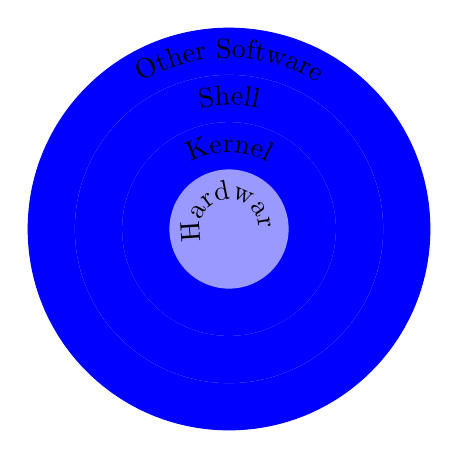
\begin{tikzpicture}[scale=0.75]
      \coordinate (O) at (0,0);
      \draw[fill=blue!10,blue!10] (O) circle (3.4);
      \onslide<4>{\draw[fill=blue,blue] (O) circle (3.4);}
      \draw[fill=blue!20,blue!20] (O) circle (2.6);
      \onslide<3>{\draw[fill=blue,blue] (O) circle (2.6);}
      \draw[fill=blue!30,blue!30] (O) circle (1.8);
      \onslide<2>{\draw[fill=blue,blue] (O) circle (1.8);}
      \draw[fill=blue!40,blue!40] (O) circle (1.0);

      \draw[decoration={text along path,reverse path,text align={align=center},text={Other Software}},decorate] (2.9,0) arc (0:180:2.9);
      \draw[decoration={text along path,reverse path,text align={align=center},text={Shell}},decorate] (2.1,0) arc (0:180:2.1);
      \draw[decoration={text along path,reverse path,text align={align=center},text={Kernel}},decorate] (1.3,0) arc (0:180:1.3);
      \draw[decoration={text along path,reverse path,text align={align=center},text={Hardware}},decorate] (0.5,0) arc (0:180:0.5);
    \end{tikzpicture}
  \end{columns}
\end{frame}
  
%\begin{frame}
%  \frametitle{Types of Shell}
%    \begin{itemize}
%      \item[\texttt{sh}]: Bourne Shell
%      \begin{enumerate}
%        {%\scriptsize
%          \item[$\vardiamond$] Developed by Stephen Bourne at AT\&T Bell Labs
%        }
%      \end{enumerate}
%      \item[\texttt{csh}]: C Shell
%      \begin{enumerate}
%        {%\scriptsize
%          \item[$\vardiamond$] Developed by Bill Joy at University of California, Berkeley
%        }
%      \end{enumerate}
%      \item[\texttt{ksh}]: Korn Shell
%      \begin{enumerate}
%        {%\scriptsize
%          \item[$\vardiamond$] Developed by David Korn at AT\&T Bell Labs
%          \item[$\vardiamond$] backward-compatible with the Bourne shell and includes many features of the C shell
%        }
%      \end{enumerate}
%      \item[\texttt{bash}]: Bourne Again Shell
%      \begin{enumerate}
%        {%\scriptsize
%          \item[$\vardiamond$] Developed by Brian Fox for the GNU Project as a free software replacement for the Bourne shell (sh).
%          \item[$\vardiamond$] Default Shell on Linux and Mac OSX
%          \item[$\vardiamond$] The name is also descriptive of what it did, bashing together the features of sh, csh and ksh
%        }
%      \end{enumerate}
%      \item[\texttt{tcsh}]: TENEX C Shell
%      \begin{enumerate}
%        {%\scriptsize
%          \item[$\vardiamond$] Developed by Ken Greer at Carnegie Mellon University 
%          \item[$\vardiamond$] It is essentially the C shell with programmable command line completion, command-line editing, and a few other features.
%        }
%      \end{enumerate}
%    \end{itemize}
%\end{frame}

%\begin{frame}
%  \frametitle{Shell Comparison}
%  \begin{columns}
%    \column{0.65\textwidth}
%    \begin{center}
%      \begin{tikzpicture}
%        \node (tbl) {
%          \begin{tabularx}{\textwidth}{cccccc}
%            \arrayrulecolor{black}
%            \textcolor{white}{\textbf{Software} }& \textcolor{white}{\textbf{sh}} &\textcolor{white}{\textbf {csh}} & \textcolor{white}{\textbf{ksh}} & \textcolor{white}{\textbf{bash}} & \textcolor{white}{\textbf{tcsh}} \\
%            Programming Language\rule{0pt}{3.5ex} & \cmark & \cmark & \cmark & \cmark & \cmark \\
%            Shell Variables & \cmark & \cmark & \cmark & \cmark & \cmark \\
%            Command alias & \xmark & \cmark & \cmark & \cmark & \cmark \\
%            Command history & \xmark & \cmark & \cmark & \cmark & \cmark \\
%            Filename completion & \xmark & \smark & \smark & \cmark & \cmark \\
%            Command line editing & \xmark & \xmark & \smark & \cmark & \cmark \\
%            Job control & \xmark & \cmark & \cmark & \cmark & \cmark \\
%            [1.0ex]
%        \end{tabularx}};
%        \begin{pgfonlayer}{background}
%          %\draw[rounded corners,top color=blue!30!black,bottom color=blue!10!white,
%          \draw[rounded corners,top color=lupurple,bottom color=lupurple,
%            draw=lubrown!30] ($(tbl.north west)+(0.14,0)$)
%          rectangle ($(tbl.north east)-(0.13,0.9)$);
%          %\draw[rounded corners,top color=black,bottom color=lubrown!20,
%          %   middle color=lubrown!20,draw=lubrown!20] ($(tbl.south west)
%          %   +(0.12,0.5)$) rectangle ($(tbl.south east)-(0.12,0)$);
%          %\draw[rounded corners,top color=green!5,bottom color=green!5,draw=green!5]
%          \draw[rounded corners,top color=lulime,bottom color=lulime,draw=lulime]
%          ($(tbl.north east)-(0.13,0.6)$)
%          rectangle ($(tbl.south west)+(0.13,0.2)$);
%        \end{pgfonlayer}
%      \end{tikzpicture}
%      \begin{itemize}
%        \item[\cmark]: Yes
%        \item[\xmark]: No
%        \item[\smark]: Yes, not set by default
%        \item[] {\fontsize{6}{7}\selectfont\url{http://www.cis.rit.edu/class/simg211/unixintro/Shell.html}}
%      \end{itemize}
%    \end{center}
%  \end{columns}
%\end{frame}

%\begin{frame}
%  \frametitle{\small Start Up Scripts}
%  \begin{itemize}
%    \item When you login to a *NIX computer, shell scripts are automatically loaded depending on your default \textbf{\color{lubrown}shell}
%    \item \textbf{\color{lubrown}sh,ksh}
%    \begin{enumerate}
%        \item \texttt{\color{blue}/etc/profile}
%        \item \texttt{\color{blue}\$HOME/.profile}
%    \end{enumerate}
%    \item \textbf{\color{lubrown}bash}
%    \begin{enumerate}
%        \item \texttt{\color{blue}/etc/profile}, login terminal only
%        \item \texttt{\color{blue}/etc/bashrc} or \texttt{\color{blue}/etc/bash/bashrc}
%        \item \texttt{\color{blue}\$HOME/.bash\_profile}, login terminal only
%        \item \texttt{\color{blue}\$HOME/.bashrc}
%    \end{enumerate}
%    \item \textbf{\color{lubrown}csh,tcsh}
%    \begin{enumerate}
%        \item \texttt{\color{blue}/etc/csh.cshrc}
%        \item \texttt{\color{blue}\$HOME/.tcshrc}
%        \item \texttt{\color{blue}\$HOME/.cshrc} if .tcshrc is not present
%    \end{enumerate}
%    \item The \texttt{\color{blue}.bashrc, .tcshrc, .cshrc, .bash\_profile} are script files where users can define their own aliases, environment variables, modify paths etc.
%    %\item e.g. the \textbf{\color{lubrown}alias} command covered earlier can be put in one of these script files depending on your \textbf{\color{lubrown}shell}
%  \end{itemize}
%\end{frame}

%\begin{frame}[fragile, allowframebreaks]
%  \frametitle{\small Examples}
%  \begin{lstlisting}[language=bash,basicstyle=\tiny\ttfamily]
%# .bashrc
%
%# Source global definitions
%if [ -f /etc/bashrc ]; then
%        . /etc/bashrc
%fi
%
%# User specific aliases and functions
%alias c="clear"
%alias rm="/bin/rm -i"
%alias psu="ps -u apacheco"
%alias em="emacs -nw"
%alias ll="ls -lF"
%alias la="ls -al"
%export PATH=/home/apacheco/bin:${PATH}
%export g09root=/home/apacheco/Software/Gaussian09
%export GAUSS_SCRDIR=/home/apacheco/Software/scratch
%source $g09root/g09/bsd/g09.profile
%
%export TEXINPUTS=.:/usr/share/texmf//:/home/apacheco/LaTeX//:${TEXINPUTS}
%export BIBINPUTS=.:/home/apacheco/TeX//:${BIBINPUTS}
%  \end{lstlisting}
%
%  \begin{lstlisting}[language=csh,basicstyle=\tiny\ttfamily]
%# .tcshrc
%
%# User specific aliases and functions
%alias c clear
%alias rm "/bin/rm -i"
%alias psu "ps -u apacheco"
%alias em "emacs -nw"
%alias ll "ls -lF"
%alias la "ls -al"
%setenv PATH "/home/apacheco/bin:${PATH}"
%setenv g09root "/home/apacheco/Software/Gaussian09"
%setenv GAUSS_SCRDIR "/home/apacheco/Software/scratch"
%source $g09root/g09/bsd/g09.login
%
%setenv TEXINPUTS ".:/usr/share/texmf//:/home/apacheco/LaTeX//:${TEXINPUTS}"
%setenv BIBINPUTS ".:/home/apacheco/TeX//:${BIBINPUTS}"
%  \end{lstlisting}
%\end{frame}

\begin{frame}
  \frametitle{Files and Processes}
  \begin{itemize}
    \item Everything in Linux/UNIX is either a file or a process
    \item A File is a collection of data, created by users using text editors, running compilers, etc.
    \item Examples of Files:
    \begin{enumerate}
      {%\scriptsize
        \item document such as collection of ascii text as in report, essay, etc. 
        \item program written in some high level programming language
        \item instructions comprehensible to machine but not a casual user such as executable, binary file
        \item directory containing information about its contents such as subdirectories or other files
      }
    \end{enumerate}
    \item A process is an executing program identified by a unique process identifier or PID.
  \end{itemize}
\end{frame}

%% Tikz File System Heirarchy
 \tikzset{
    invisible/.style={opacity=0},
    visible on/.style={alt={#1{}{invisible}}},
    alt/.code args={<#1>#2#3}{%
      \alt<#1>{\pgfkeysalso{#2}}{\pgfkeysalso{#3}} % \pgfkeysalso doesn't change the path
    },
  }

\begin{frame}{File System Hierarchy}
\tikzset{every node/.append style={scale=0.4}}

\begin{tikzpicture}[scale=0.4]
  \path[mindmap,concept color=lubrown,text=lucream,
  level 1 concept/.append style={every child/.style={concept color=luorange,text=black},sibling angle=-15},
  level 2 concept/.append style={every child/.style={concept color=luorange2,text=black}, sibling angle=-40},
  level 3 concept/.append style={every child/.style={concept color=lulime,text=black}}]
    node[concept] {root directory (/)}
    [clockwise from=180]
    child[style={concept}, level distance=8.5cm, visible on=<2->] { node[concept] {bin}}
    child[concept, visible on=<3->] { node[concept] {boot}}
    child[style={concept}, level distance=8.5cm, visible on=<4->] { node[concept] {dev}}
    child[concept, visible on=<5->] { node[concept] {etc}}
    child[style={concept}, level distance=8.5cm, visible on=<6->] { node[concept] {home}
		[counterclockwise from=-90]
      	child { node[concept] {alp514} 
        	[clockwise from=0]
            child { node[concept] {.bashrc}}
            child { node[concept] {bin}}
            child { node[concept] {Documents}}
            child { node[concept] {packages}}
            child { node[concept] {$\cdots$}}
        }
      	child[visible on=<16->] { node[concept] {sma310} }
      	child[visible on=<16->] { node[concept] {$\cdots$} }
	}
    child[concept, visible on=<7->] { node[concept] {lib64 \& lib}}
    child[style={concept}, level distance=8.5cm, visible on=<8->] { node[concept] {mnt}}
    child[concept, visible on=<9->] { node[concept] {proc}}
    child[style={concept}, level distance=8.5cm, visible on=<10->] { node[concept] {sbin}}
    child[concept, visible on=<11->] { node[concept] {tmp}}
    child[style={concept}, level distance=11.5cm, visible on=<12->] { node[concept] {usr}
		[counterclockwise from=15]
      	child { node[concept] {bin} }
      	child { node[concept] {lib64 \& lib} }
      	child { node[concept] {local} }
      	child { node[concept] {include} }
      	child { node[concept] {sbin} }
      	child { node[concept] {share} }
        }
    child[concept, visible on=<13->] { node[concept] {var}}
    child[style={concept}, level distance=8.5cm, visible on=<14->] { node[concept] {zhome}
		[counterclockwise from=0]
      	child { node[concept] {Apps} 
        	[clockwise from=50]
            child { node[concept] {matlab}}
            child { node[concept] {gcc}}
            child { node[concept] {intel}}
            child { node[concept] {pgi}}
        }
      	child { node[concept] {alp514} }
      	child { node[concept] {sma310} }
      	child { node[concept] {$\cdots$} }
	}
;
\end{tikzpicture}

\begin{itemize}
\only<1>{\item All files are arranged in a hierarchial structure, like an inverted tree.}
\only<1>{\item The top of the hierarchy is traditionally called \textbf{root} (written as a slash / )}
\only<2>{\item contains files that are essential for system operation, available for use by all users.}
\only<3>{\item contains bootable kernel and bootloader}
\only<4>{\item contains various devices such as hard disk, CD-ROM drive etc}
\only<5>{\item contains various system configurations}
\only<6>{\item contains home directories of all users. This is the directory where you are at when you login to a Linux/UNIX system.}
\only<7>{\item contains libraries that are essential for system operation, available for use by all users.}
\only<8>{\item directories where disk drives are mounted}
\only<9>{\item process information pseudo-file system containing runtime system information (e.g. system memory, devices mounted, hardware configuration, etc).}
\only<9>{\item can be regarded as a control and information centre for the kernel.}
\only<10>{\item same as bin but only accessible by \textbf{root}}
\only<11>{\item temporary file storage}
\only<12>{\item contains user documentations, binaries, libraries etc}
\only<13>{\item used to store files which change frequently (system level not user level)}
\only<14>{\item where we install applications common to all HPC systems}
\only<15>{\item Installing your own OS: /bin,/lib\{64\},/etc,/dev and /sbin must be on the same partition.}
\only<16>{\item UNIX like OS's are designed for multi user environments i.e. multiple users can exist on the system.}
\only<16>{\item Special user called \textbf{root} is the administrator and has access to all files in the system.}
\end{itemize}
\end{frame}



%\begin{frame}
%  \frametitle{Important Directories}
%  \begin{description}
%    \item[/bin:] contains files that are essential for system operation, available for use by all users.
%    \item[/lib,/lib64:] contains libraries that are essential for system operation, available for use by all users.
%    \item[/var:] used to store files which change frequently (system level not user level)
%    \item[/etc:] contains various system configurations
%    \item[/dev:] contains various devices such as hard disk, CD-ROM drive etc
%    \item[/sbin:] same as bin but only accessible by \textbf{root}
%    \item[/tmp:] temporary file storage
%    \item[/boot:] contains bootable kernel and bootloader
%    \item[/usr:] contains user documentations, binaries, libraries etc
%    \item[/home:] contains home directories of all users. This is the directory where you are at when you login to a Linux/UNIX system.
%  \end{description}
%  \begin{itemize}
%    \item Installing your own OS: /bin,/lib\{64\},/etc,/dev and /sbin must be on the same partition.
%  \end{itemize}
%\end{frame}

%\begin{frame}[fragile]
%  \frametitle{\small }
%  \begin{itemize}
%    \item UNIX like OS's are designed for multi user environments i.e. multiple users can exist on the system.
%    \item Special user called \textbf{root} is the administrator and has access to all files in the system.
%    \item In *nix, users are organized into groups.
%    \item Each user is in alteast one group.
%    \item Group membership makes it easier to share files with members of your group.
%    \item[]Type \Verblubrown{groups{\Enter}} to find your group membership.
%    \item All files are \textit{case sensitive},
%    \item[$\vardiamond$] myfile.txt, Myfile.txt and myfile.TXT are three different files and can exist in the same directory simultaneously.
%  \end{itemize}
%\end{frame}

\section{Live Demo}
\begin{frame}{openSUSE KDE Desktop}
  \begin{center}
    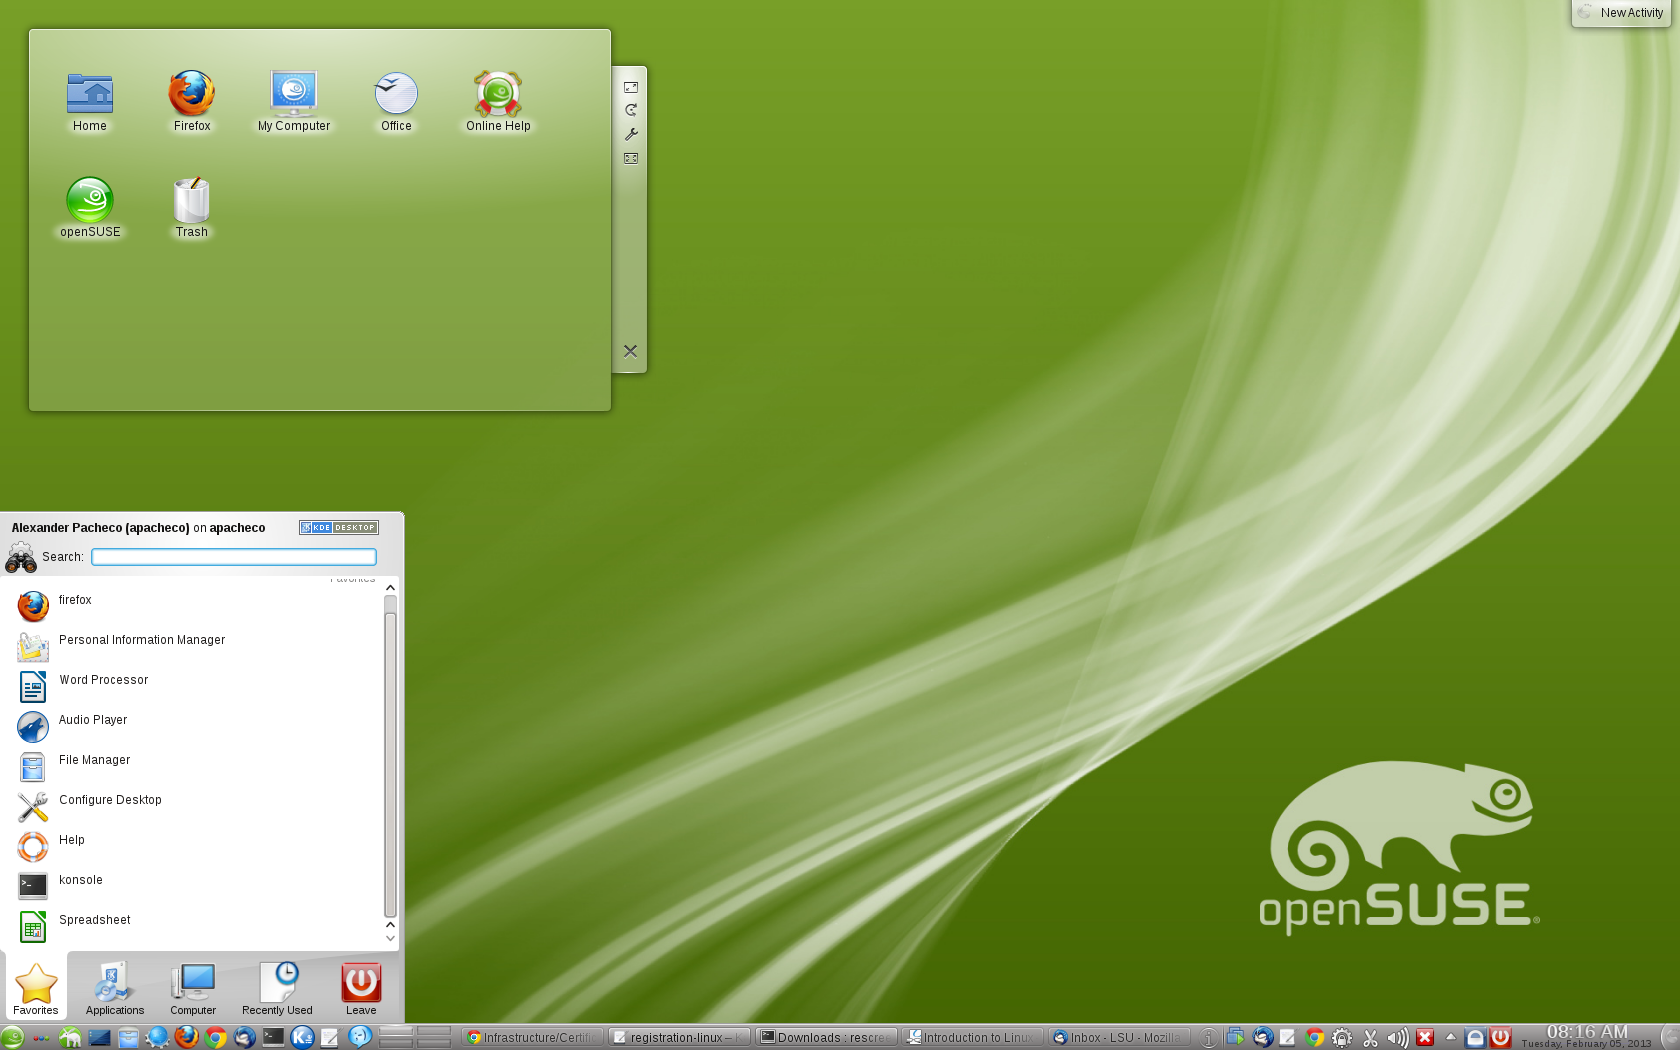
\includegraphics[width=\textwidth]{./opensuse}
  \end{center}
\end{frame}
\begin{frame}{openSUSE Awesome Dynamic Window Manager}
  \begin{center}
    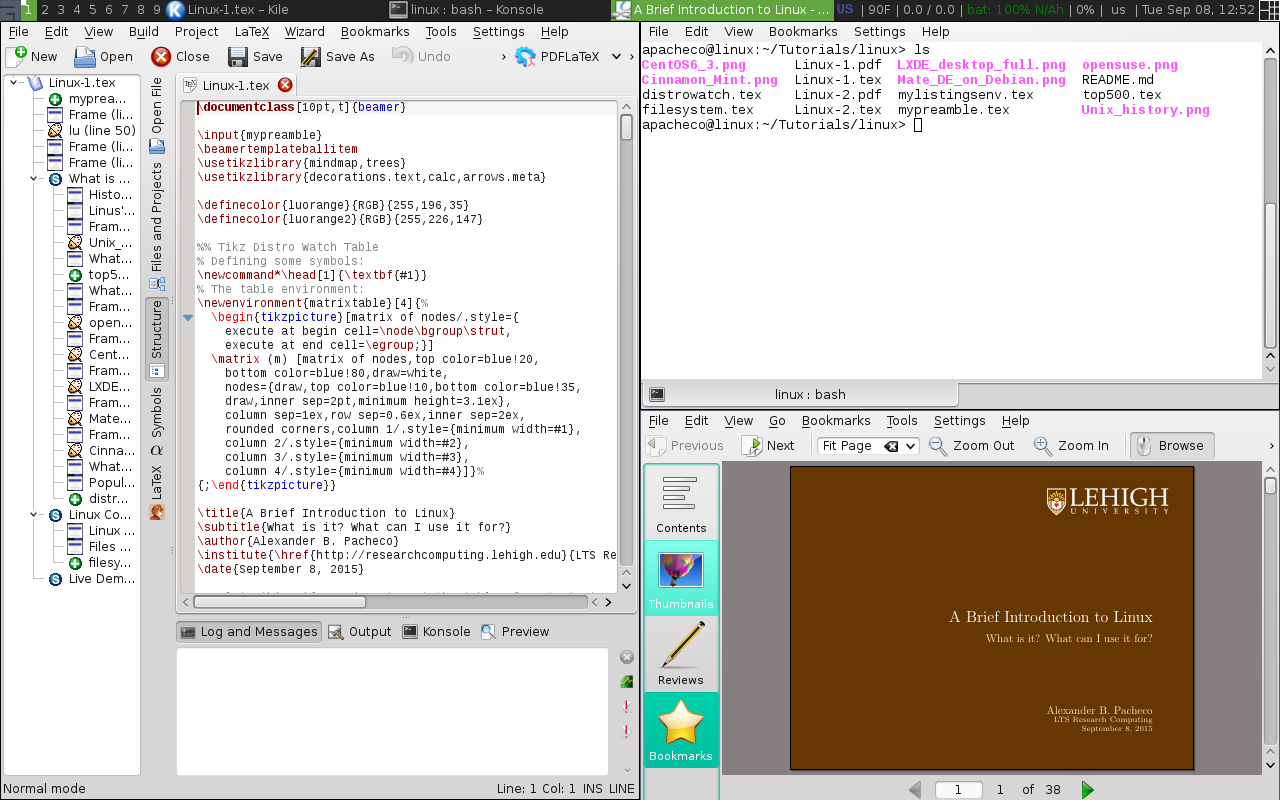
\includegraphics[width=\textwidth]{./opensuse-awesome}
  \end{center}
\end{frame}
\begin{frame}{openSUSE GNOME}
  \begin{center}
    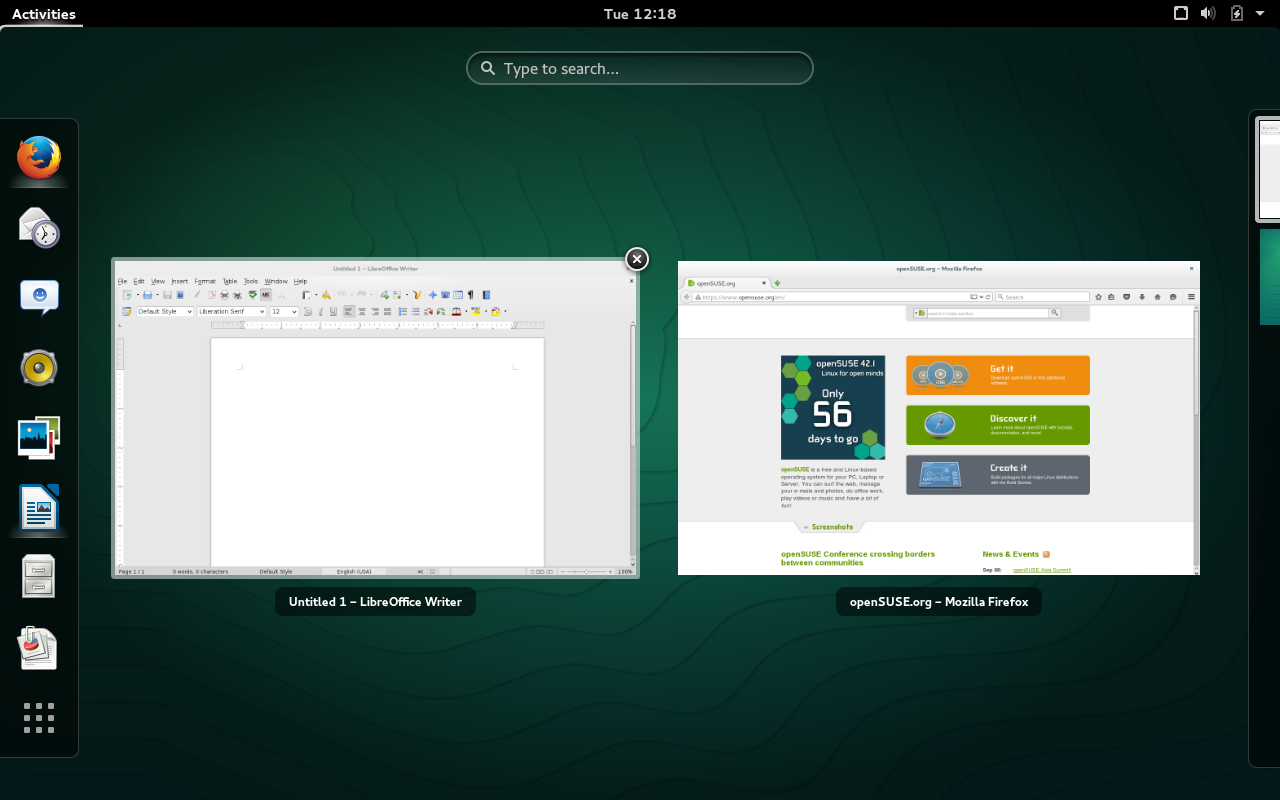
\includegraphics[width=\textwidth]{./opensuse-gnome}
  \end{center}
\end{frame}
\begin{frame}{CentOS GNOME Desktop}
  \begin{center}
    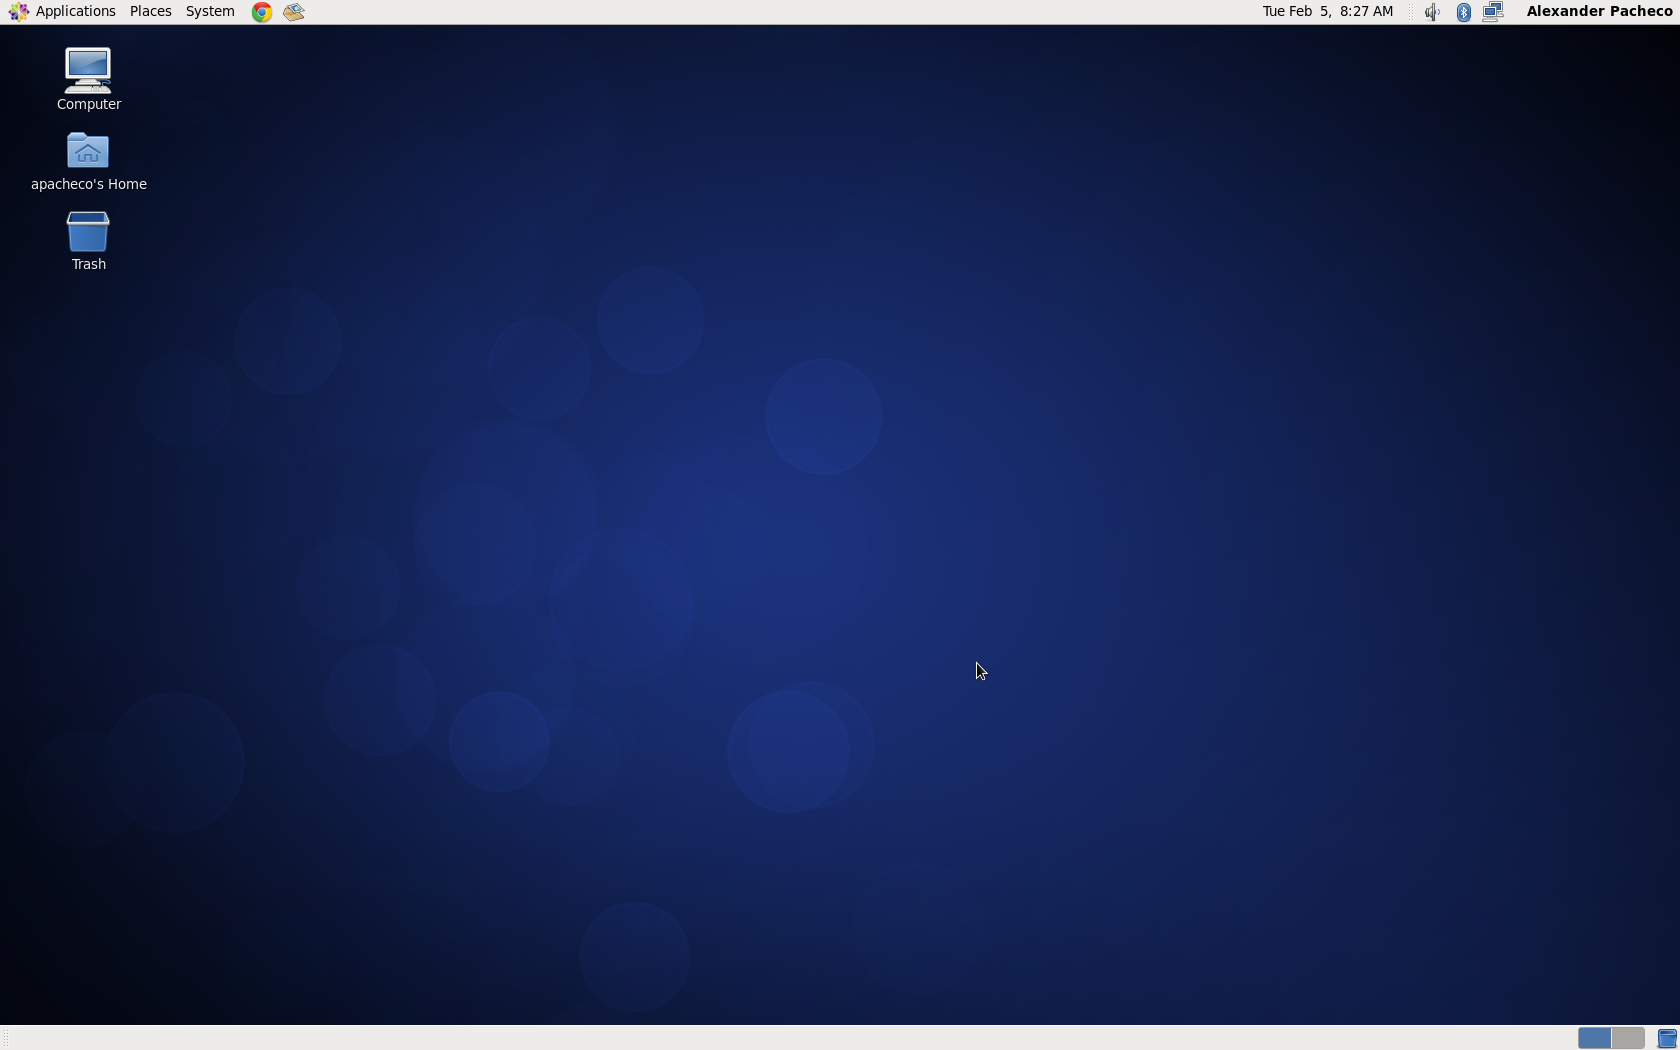
\includegraphics[width=\textwidth]{./CentOS6_3}
  \end{center}
\end{frame}
\begin{frame}{Ubuntu Unity Desktop}
  \begin{center}
    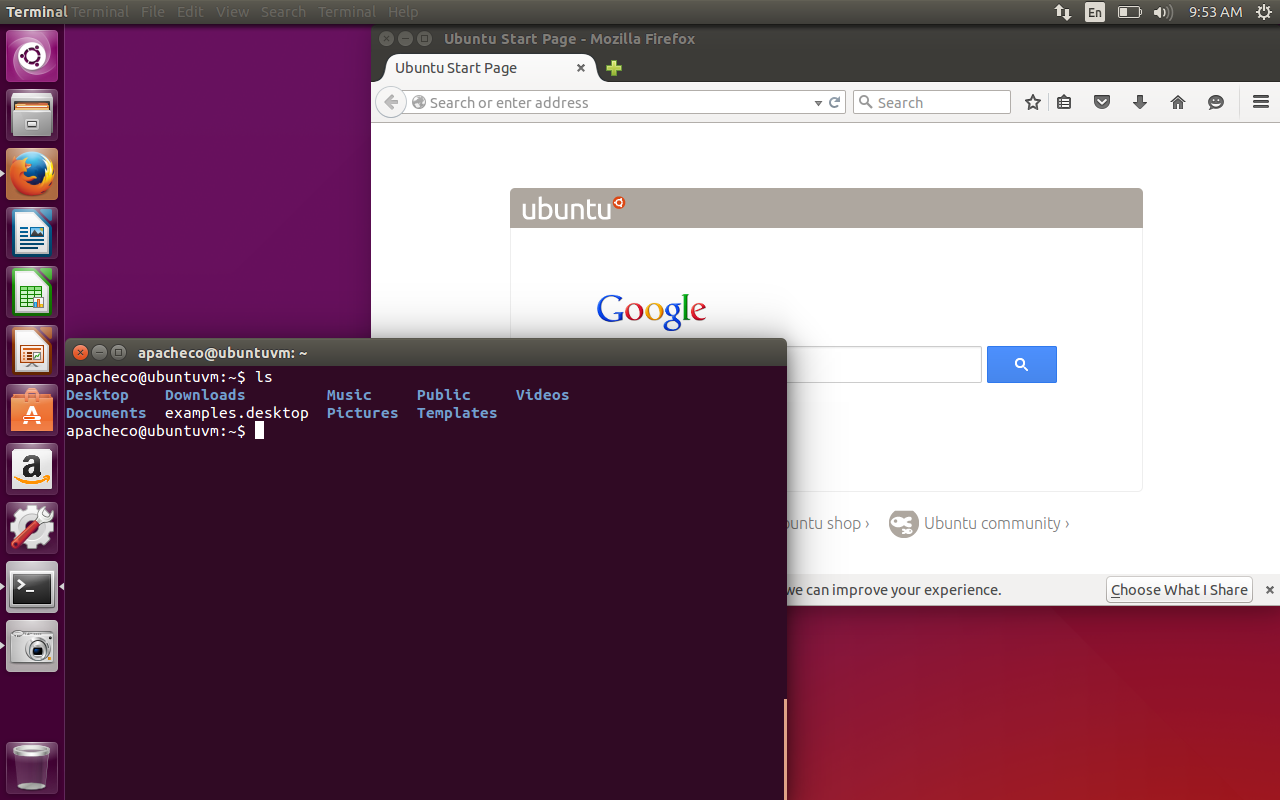
\includegraphics[width=\textwidth]{./Ubuntu}
  \end{center}
\end{frame}
\begin{frame}{Linux Mint Debian Edition MATE Desktop}
  \begin{center}
    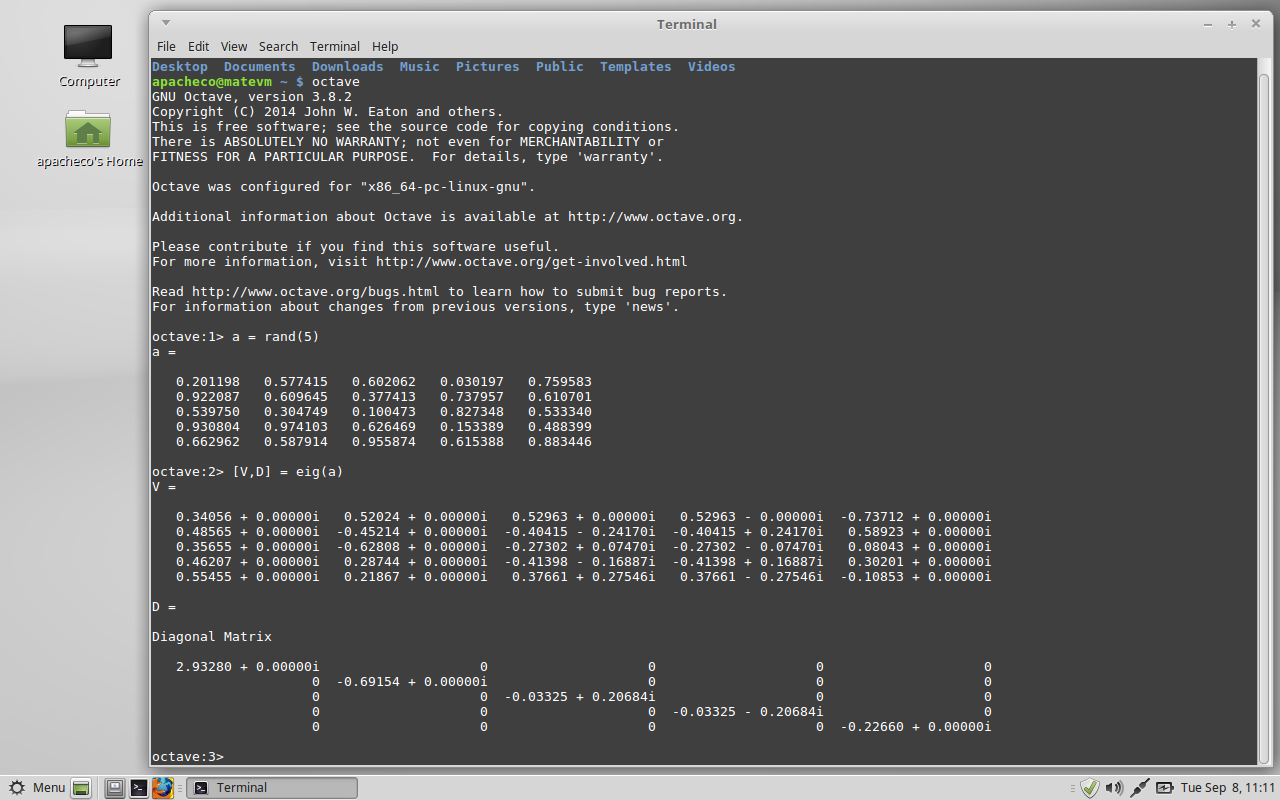
\includegraphics[width=\textwidth]{./mate}
  \end{center}
\end{frame}
\begin{frame}{Linux Mint Cinnamon Desktop}
  \begin{center}
    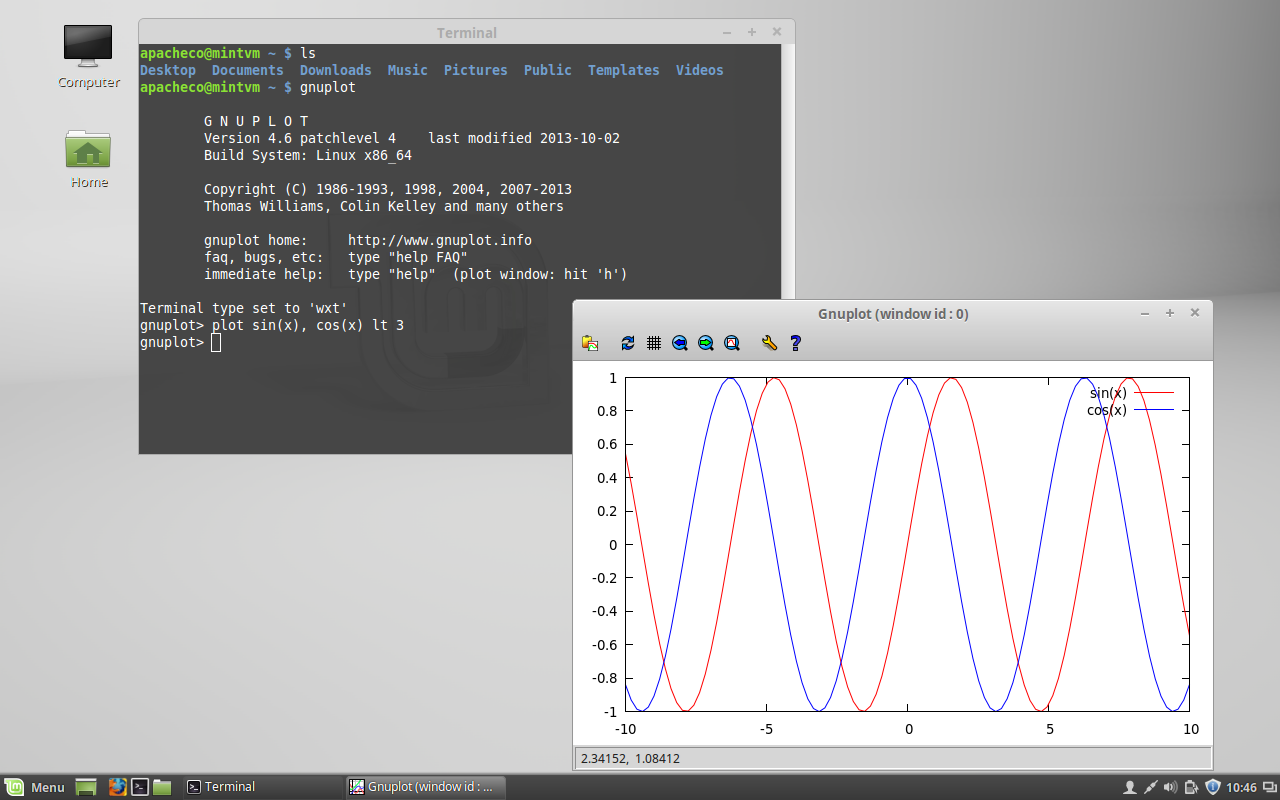
\includegraphics[width=\textwidth]{./mint}
  \end{center}
\end{frame}
\begin{frame}{Lubuntu LXDE Desktop}
  \begin{center}
    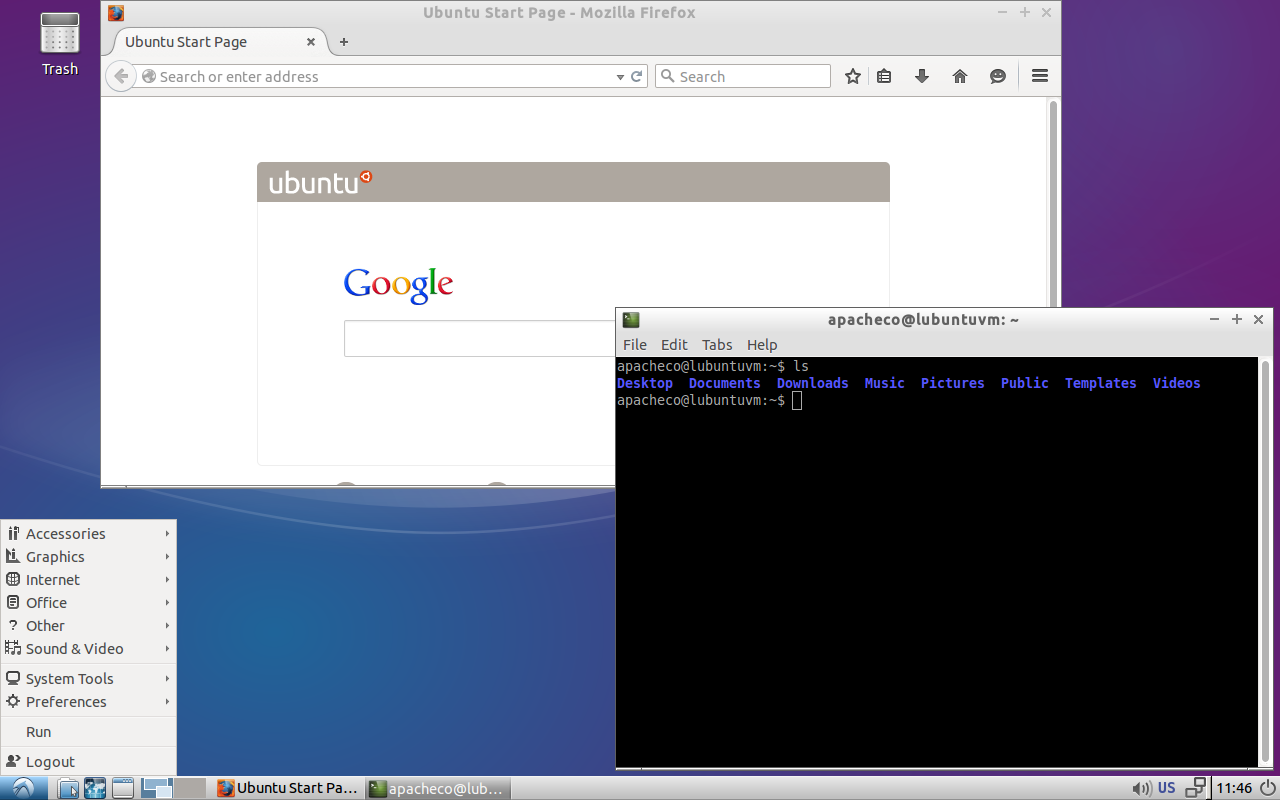
\includegraphics[width=\textwidth]{./lubuntu}
  \end{center}
\end{frame}
\begin{frame}{Xubuntu Xfce Desktop}
  \begin{center}
    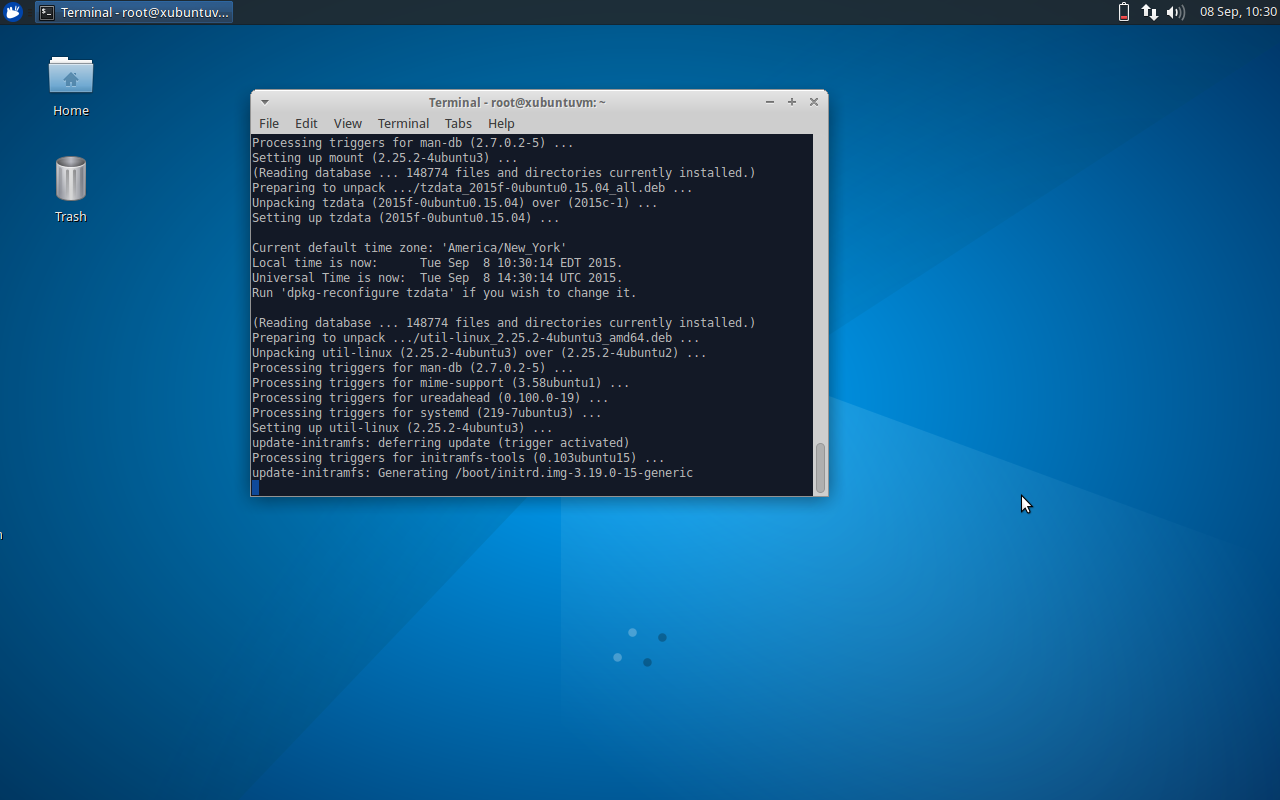
\includegraphics[width=\textwidth]{./xubuntu}
  \end{center}
\end{frame}
\begin{frame}{FreeBSD (Unix not Linux) Awesome DWM}
  \begin{center}
    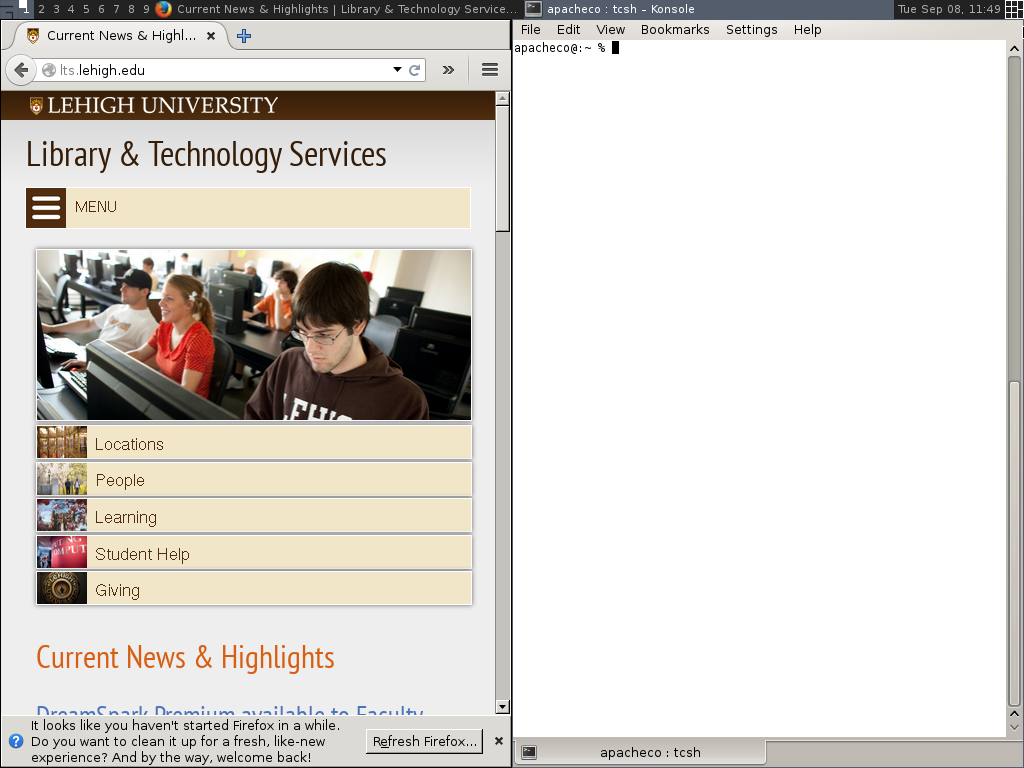
\includegraphics[width=0.8\textwidth]{./freebsd}
  \end{center}
\end{frame}

\end{document}

